\documentclass[msc,proposal,hidelot,hideabstract]{ppgccufmg} % ou [msc] para dissertações
                                        % de mestrado. Para propostas ou
                                        % projetos, usar [phd,project],
                                        % [msc,proposal], etc.
\usepackage[brazil]{babel} % ajusta vários detalhes para
                           % documentos escritos em português,
                           % principalmente hifenização
\usepackage[T1]{fontenc}   % permite a hifenização de
                           % palavras acentuadas
\usepackage[utf8x]{inputenc} % ou [utf8x] para quem prefere
                             % usar a codificação UTF-8
\usepackage{graphicx} % define o comando \includegraphics
                      % para a inclusão de Figuras
%\usepackage[square]{natbib} % permite citações naturalmente
                            % integradas ao texto
\usepackage[a4paper,
portuguese,
bookmarks=true,
bookmarksnumbered=true,
linktocpage,
colorlinks=true,
citecolor=black,
urlcolor=black,
linkcolor=black,
filecolor=black,
]{hyperref}
\usepackage[table,xcdraw]{xcolor}
\usepackage{amsmath}
\begin{document}
\ppgccufmg{
title={Uma Metodologia para\\
Recomendação de \\
Requisições de Mudanças \\
Similares},
author={Vagner Clementino dos Santos},
university={Universidade Federal de Minas Gerais},
course={Ciência da Computação},
address={Belo Horizonte},
date={2015-11},
advisor={Rodolfo F. Resende},
abstract={Resumo}{resumo},
}
\chapter{Introdução}
\label{ch:intro}
Dentro do ciclo de vida do produto de software o processo de manutenção tem
papel fundamental. Apesar de não ter merecido tanta atenção quanto a parte de
projeto e desenvolvimento de software, no últimos anos o processo de manter o
software vem ganhando relevância devido, primordialmente, à seu custo
associado.

No Capítulo \ref{ch:justificativa} . O Capítulo \ref{ch:revisao} . No
Capítulo \ref{ch:metodologia} é discutida a metologia a ser aplicada. No
Capítulo \ref{ch:conclusao_trab_futuros}, especialmente na Tabela \ref{tab:cronograma} é exibido o cronograma do trabalho.

\chapter{Justificativa}
\label{ch:justificativa}
Desde o final da década de 1970 \cite{Zelkowitz:1979:PSE:578504}  percebe-se o aumento do custo referente as
atividades de  manutenção de software.
%Na Tabela \ref{tab:software-cost}, adaptada de  \cite{koskinen2003software},
%é possível verificar esta tendência.
Em um trabalho mais recente \cite{1423995}, Yong \& Mookerjee propõe um modelo que reduz o custos de
manutenção e reposição durante a vida útil de um sistema de software. O modelo
proposto demonstrou quem em algumas situações é \textit{melhor substituir um
  sistema do que mantê-lo}. Com o objetivo de mensurar o custo do software
algum trabalhos vêm desenvolvendo novos modelos a fim de melhorar a acurácia
dos valores obtidos. Alguns destes trabalhos descrevem que o custo para manter
um sistema pode chegar a 60\% \cite{kaur2015review}. Este mesmo percentual
refere-se ao total de desenvolvedores dedicados à tarefas de manutenção de
sistemas \cite{Zhang_2003}. Neste contexto, existe também por parte da acadêmia quando da
industria o interesse no desenvolvimento de técnicas que reduzem o esforço das
tarefas de manutenção de software ao mesmo tempo que reduza o seu custo.

%\begin{table}[ht]
%\resizebox{\textwidth}{!}{%
%\begin{tabular}{|c|c|c|c|}
%\hline
%\rowcolor[HTML]{FFFFFF}
%\textbf{Ano} & \textbf{Proporção} & \multicolumn{1}{c|}{\cellcolor[HTML]{FFFFFF}\textbf{Metodologia}} & \multicolumn{1}{c|}{\cellcolor[HTML]{FFFFFF}\textbf{Referência}} \\ \hline
%2000 & \textgreater90\% & $\frac{\text{(Custo com manutenção e evolução do software)}}{\text{(Custo total do software)}}$ &\cite{846201} \\ \hline
%1993 & 75\% & $\frac{\text{(Manutenção de Software)}}{\text{(Orçamento com Sistemas de Informação)}}$ & \cite{swe.cost.legacy2}\\ \hline
%1990 & \textgreater90\% & $\frac{\text{(Custo com manutenção de sistema)}}{\text{(Custo total com Software)}}$ & \cite{moad1990maintaining}\\ \hline
%1988 & 60-70\% & $\frac{\text{(Manutenção de software)}}{\text{(Orçamento com a operação de Sistemas de Gerenciamento da Informação)}}$ & \cite{Port1988}\\ \hline
%1984 & 65-75\% & $\frac{\text{(Esforço gasto em manutenção de software)}}{\text{(Tempo total disponível para esforço em Engenharia de Software)}}$ & \cite{McKee:1984:MFD:1499310.1499334}\\ \hline
%1981 & 50\% & $\frac{\text{(Tempo gasto com manutenção de software)}}{\text{(Tempo Total)}}$ & \cite{Lientz:1981:PAS:358790.358796}\\ \hline
%1979 & 67\% & $\frac{\text{(Custo com Manutenção)}}{\text{(Custo Total com Software)}}$ & \cite{Zelkowitz:1979:PSE:578504}\\ \hline
%\end{tabular}
%}
%\caption{Proporção do Custo de Manutenção de Software. Adaptado de \cite{koskinen2003software}}
%\label{tab:software-cost}
%\end{table}
%

Uma possível forma de reduzir o custo de manutenção de um sistema de software é
aumentar a produtividade do desenvolvedor devotado às atividade de
manutenção. No contexto do processo de desenvolvimento de software tradicional,
conforme supõe a \textit{ISO/IEC 14764} \cite{1703974}, a manutenção de
software pode estruturada conforme a Figura \ref{fig:maintence-process}.

\begin{figure}[hbtp]
\centering
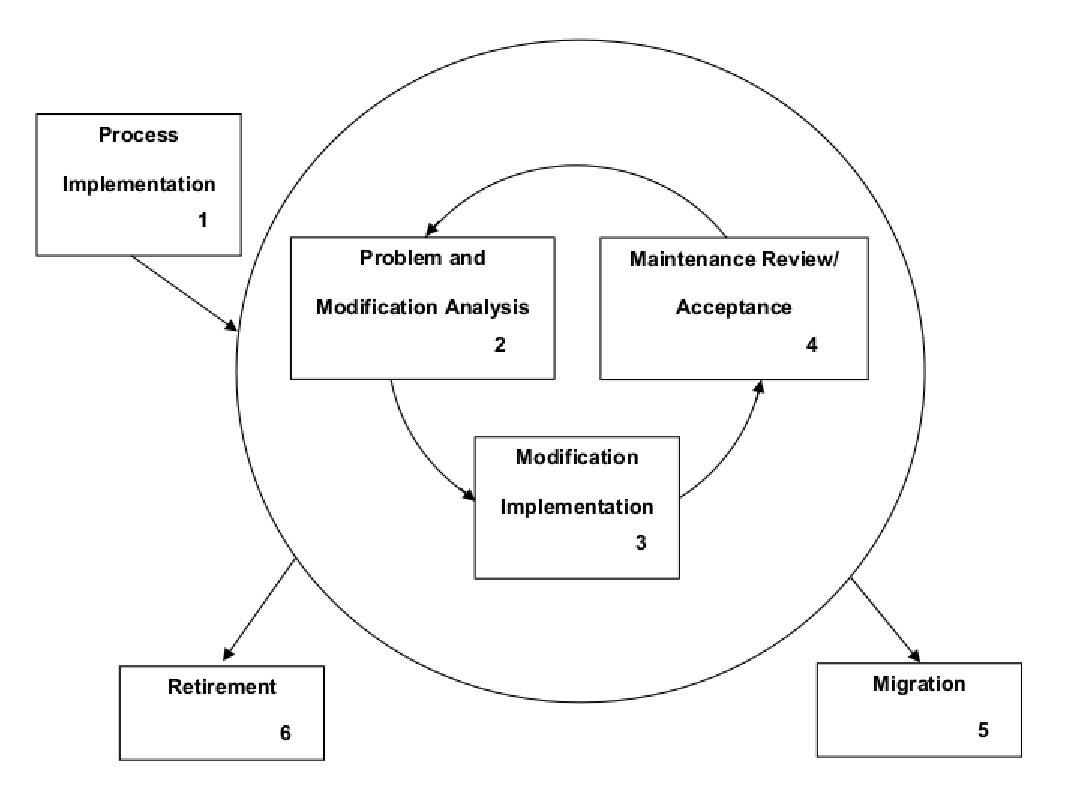
\includegraphics[width=.75\textwidth]{../img/maintence_process.eps}
\caption{Processo de manutenção de software da norma ISO/IEC 14764. Adaptado: \cite{1703974}}
\label{fig:maintence-process}
\end{figure}

Na atividade \textit{1 - Implementação do processo (Process
Implementation)} os planos e procedimentos a serem executados
durante a fase de manutenção devem ser estabelecidos e aprovados. Muitos o
plano proposto define o processo de atribuição das MR's para os
desenvolvedores. Esta tomada de decisão geralmente leva em conta a prioridade
do serviço a ser realizado, as habilidades do programador dentre outros
critérios. Todavia, este processo poderia obter melhores resultados se a cada
Requisição atribuída a um desenvolvedor, outras similares, também pudessem ser
sugeridas.


Tal tomada de decisão apoiada por alguma metodologia para recomendar MR's
similares trará os seguinte benefícios:

\begin{itemize}
\item \textit{Redução da troca de contexto (context switch)};
\item \textit{Aumento da produtividade};
\item \textit{Melhorar a qualidade das MR's sugeridas através de uma técnica mais
  potente do que aquelas da Recuperação da Informação}.
\end{itemize}

Com o objetivo de mensurar o custo relativo à manutenção de software
\cite{benaroch2013primary,5873461,ren2011research}, bem com melhoria as
atividades relacionadas ao processo de manutenção  mediante a proposição
de modelos \cite{April200973}, \cite{930170} e \cite{5741246} diversos
trabalhos vêm sendo propostos. Nesta mesma linha de pesquisa, alguns estudo
focam na melhoria da produtividade do desenvolvedor através de ações como a remoção de Requisições de Mudança -
Modification Request (MR) duplicadas
\cite{Alipour:2013:CAT:2487085.2487123,6671283,09639314} ou ainda recomendando
MR's similares que reduzem a mudança de contexto (context switch) \cite{5741246,101186}.

Em geral, afim de remover duplicadas ou sugerir MR's similares são utilizadas de
técnicas de Recuperação da Informação - Information Retrieve
\cite{baeza1999modern} tomando como base a descrição textual da Requisição \cite{101186,Runeson:2007:DDD:1248820.1248882}. Apesar dos resultados
relevantes obtidos por esta técnica verifica-se que ela é fortemente
dependente da forma que o solicitante da MR descreve a sua requisição. Além disso
há problema dos sinônimos, em que demandas similares mas, escritas com palavras
diferentes, podem não ser recuperadas.

Neste contexto é proposto uma ferramenta para recomendação de Requisições de
Mudanças similares utilizando Redes Neurais.

O problema de recomendar Requisições de Mudanças similares pode ser definido
formalmente conforme segue:

Seja $I$ o conjunto de Requisições de Mudanças (MR) em aberto para um
sistema $S$ qualquer. A cardinalidade de $I$ é dada por $n$. Seja $i$ um MR,
tal que $i \in I$, que foi atribuída para um desenvolver
$d$. Pede-se que seja encontrado um subconjunto $J \subset I$, de tamanho $k \ll n$, tal
que para todo $j$, tal que $j \in J$, seja similar a $i$ em um grau maior ou igual a
$s$. Onde $s$ é limiar inferior de similaridade. Neste caso, o problema se resume em
encontrar uma função de similaridade a ser aplicada a cada elemento $m \in I$,
onde $m \neq i$.

\chapter{Revisão da Literatura}
\label{ch:revisao}

No trabalho de Junio et al. \cite{5741246} é proposto um processo denominado PASM (Process for Arranging
Software Maintenance Requests) que propõe lidar com tarefas de manutenção como
projetos de software. Para tanto, utilizou-se técnicas de análise de
agrupamento (clustering) a fim de melhor compreender e comparar as demandas de
manutenção. Os resultados demostraram que depois de adotar PASM os
desenvolvedores têm dedicado mais tempo para análise e validação e menos tempo
para as tarefas de execução e de codificação.

\textit{NextBug} \cite{101186} é uma extensão (plugin) para a ferramenta de Controle de Demanda -
Issue Tracking System (ITS) Bugzilla\footnote{\url{https://www.bugzilla.org/}}
que recomenda novos bugs para um desenvolvedor baseado no bug que ele esteja
tratando atualmente. O objetivo da extensão é sugerir bugs com base em técnicas de
Recuperação de Informação \cite{baeza1999modern}.

\chapter{Metodologia}
\label{ch:metodologia}

O processo de desenvolvimento deste trabalho pode ser dividido nas seguintes
etapas $I$\textit{ - Revisão Sistemática da Literatura}; $II$\textit{ - Prova de Conceito)}; $IV$\textit{ - Avaliação}. Cada uma das etapas é detalhada nas próximas seções.

\section{Revisão Sistemática da Literatura}
\label{sec:revisao_sistematica}

Uma \textit{Revisão Sistemática da Literatura} - SLR (do inglês Systematic Literature Review) é uma
metodologia científica cujo objetivo é identificar, avaliar e interpretar
\textit{toda} pesquisa \textit{relevante} sobre uma questão de pesquisa, área
ou fenômeno de interesse \cite{keele2007guidelines,wohlin2012experimentation}. Neste trabalho
será utilizada as diretrizes proposta \cite{keele2007guidelines} no qual uma
Revisão Sistemática deve seguir os seguintes passos:

\begin{enumerate}
  \item \textbf{Planejamento}
  \begin{enumerate}
    \item \textit{Identificar a necessidade da Revisão}
    \item \textit{Especificar questões de pesquisa}
    \item \textit{Desenvolver o Protocolo da Revisão}
  \end{enumerate}
  \item \textbf{Condução/Execução}
  \begin{enumerate}
    \item \textit{Seleção dos Estudos Primários}
    \item \textit{Análise da qualidade dos Estudos Primários}
     \item \textit{Extração dos Dados}
     \item \textit{Sintetização dos Dados}
   \end{enumerate}
  \item \textbf{Escrita/Publicação}
  \begin{enumerate}
    \item \textit{Redigir documento com os resultados da Revisão}
    \item \textit{Redigir documento com lições aprendidas}
  \end{enumerate}
\end{enumerate}

Com o objetivo de entender melhor o contexto do problema da sugestão de MR's
similares, será realizada uma SRL que se propõe a responder as seguintes
questões:  A SRL que será realizada visa responder as seguintes questões de
pesquisa:

\begin{itemize}
  \item \textbf{$Q1$}: Quais são os aspectos mais importantes suportados pelas
    metodologias/ferramentas de recomendação de Requisições de Mudança e
    remoção de bugs duplicados?
  \item \textbf{$Q2$}: Como as ferramentas/metodologias atualmente disponíveis
    para recomendação de Requisições de Mudança auxiliam na tomada de decisões
    durante o processo de Manutenção de Software?
  \item \textbf{$Q3$}: Quais são as metodologias/técnicas utilizadas para
    recomendação de Requisições de Mudança e bugs duplicados?
  \item \textbf{$Q5$}: Qual procedimento utilizado para avaliar a
    técnica/metodologia proposta para recomendação de Requisições de Mudança similares e
    bugs duplicados?
  \item \textbf{$Q6$}: Em qual tipo de projeto (comercial ou código-aberto) a
    metodologia/ferramenta foi aplicada?
  \item \textbf{$Q7$} : Qual processo de software (tradicional, ágil, TDD e
    etc) envolvido no contexto no qual a ferramenta/metodologia foi aplicada?
\end{itemize}



\section{Prova de Conceito}
\label{sec:prova-conceito}

Como prova de conceito da técnica proposta pretende-se construir uma que
possibilite a recomendação Requisições de Mudança similares. A proposta é que a
ferramenta utilize técnicas para detecção de similaridades que não dependam
exclusivamente da Recuperação da Informação (Information Retrieve), como por
exemplo nos trabalho propostos por  Rocha et al. \cite{101186} e Runeson et
al. \cite{Runeson:2007:DDD:1248820.1248882}. Será realizado um estudo
exploratório a fim de verificar qual técnica será mais adequada. Neste sentido
os resultados da Revisão Sistemática da Literatura (Seção \ref{sec:revisao})
ajudará neste decisão. Todavia, o trabalho de  Rocha et al. \cite{101186} fica
sendo a linha de base (baseline) deste estudo, cujo objetivo é utilizar uma
técnica apresente melhores resultados, utilizados como métricas Feedback e
Precision \cite{zimmermann2005mining}. A avaliação da ferramenta proposta como
Prova de Conceito está descrita com maiores detalhes na \ref{sec:avaliacao}.

\section{Avaliação}
\label{sec:avaliacao}

Com o objetivo de avaliar a ferramentas proposto neste trabalho será realizado um
\textit{Quasi-Experimento} \cite{wohlin2012experimentation} utilizando a base de dados de demandas de manutenção de uma empresa
de software real. O experimento consistirá de dado que uma demanda $i$ foi atribuída a um desenvolvedor $d$,
serão geradas 03 listas de sugestões: $(i)$ lista produzida pelo gerente imediato
de $d$;$(ii)$ lista feita por um desenvolver do mesmo setor de $d$; $(iii)$
gerada pela ferramenta proposta. Naturalmente o desenvolvedor não saberá a origem
de nenhum das listas.  De posse das três listas pediremos ao
desenvolvedor $d$ que informe qual delas pode reduzir a troca de contexto e
aumentar sua produtividade. Espera-se a lista proposta pela nossa ferramenta
possua o melhor desempenho na maioria dos casos.

\chapter{Conclusão e Trabalhos Futuros}
\label{ch:conclusao_trab_futuros}

Para tanto, a tabela \ref{tab:cronograma} descreve as atividades que serão realizadas para atingir este objetivo.

\begin{table}[ht]
\centering
\resizebox{\textwidth}{!}{%
\begin{tabular}{|c|l|c|c|}
\hline
\rowcolor[HTML]{EFEFEF}
\# & \multicolumn{1}{c|}{\cellcolor[HTML]{EFEFEF}\textbf{Atividade}} & \textbf{Início (MM/AAAA)} & \textbf{Término (MM/AAAA)} \\ \hline
01 & Revisão da Literatura & \textit{10/2015} & \textit{11/2015} \\ \hline
02 & Ponto de Controle 01 – Reunião com orientador sobre Revisão da Literatura & \textit{12/2016} & \textit{12/2016} \\ \hline
03 & Avaliação da Técnica de Rede Neural & \textit{01/2016} & \textit{01/2016} \\ \hline
04 & Ponto de Controle 02 – Reunião com orientador sobre a Técnica de Rede Neural & \textit{02/2016} & \textit{02/2016} \\ \hline
05 & Implementação da Ferramenta & \textit{02/2016} & \textit{04/2016} \\ \hline
06 & Ponto de Controle 03 – Avaliação da Ferramenta Avaliada & \textit{05/2016} & \textit{05/2016} \\ \hline
07 & Experimento de Avaliação da Ferramenta & \textit{05/2016} & \textit{05/2016} \\ \hline
08 & Ponto de Controle 04 – Avaliação do Experimento junto com o orientador & \textit{05/2016} & \textit{05/2016} \\ \hline
09 & Finalização do texto da dissertação & \textit{06/2016} & \textit{07/2016} \\ \hline
10 & Ponto de Controle 05 – Avaliação do texto da dissertação com o orientador & \textit{07/2016} & \textit{07/2016} \\ \hline
11 & Defesa da dissertação & \textit{07/2016} & \textit{07/2016} \\ \hline
\end{tabular}
}
\caption{Cronograma de execução do trabalho}
\label{tab:cronograma}
\end{table}

% Incluindo bibliografia:
\ppgccbibliography{../bib/bibliografia}
\end{document}
